% Section content template for individual Educative lessons
% This file contains the actual content for a specific section
% Generated from Educative API section content

% Section: How Spotify Wrapped Scales for 7M Users
% Section ID: 4733042868224000
% Section Slug: how-spotify-wrapped-scales-for-7m-users
% Generated: 2025-12-08T15:49:45.843492

Every year-end, Spotify delivers its users a gift: a beautifully personalized summary of their listening habits. From your top songs to your most-streamed genres, Spotify Wrapped transforms your music data into an engaging, shareable story.
\\
Spotify Wrapped is also a powerful product offering that users wait for each year.~
\\
The numbers speak for themselves:

\begin{itemize}
\item
\protect\phantomsection\label{c62yztrYtRJjb4gn02RE6}
100 million+ shares on social media in 2022\href{https://hightouch.com/blog/how-spotify-wrapped-works}{\textsuperscript{\ul{1}}}
\item
\protect\phantomsection\label{bM_fFxfdPtAkfAsSDS2AH}
20\% increase in Spotify downloads in 2020\href{https://www.moengage.com/blog/spotify-wrapped-2020-app-downloads-engagement/}{\textsuperscript{\ul{2}}}
\item
\protect\phantomsection\label{NuC5gfpV9BMusgcPX7LpB}
602 million users engaged across 184 countries (as of 2023)\href{https://investors.spotify.com/financials/default.aspx\#quarterly-results}{\textsuperscript{\ul{3}}}
\end{itemize}
\\
But Spotify Wrapped is more than just a successful marketing campaign; it's a time capsule of your year in music, powered by data science, machine learning, and immaculate System Design.
\\
Behind every Wrapped recap is a robust architecture that processes petabytes of data with precision and speed. This means that engineers are working diligently to ensure Wrapped is seamless, scalable, and always ready for millions of users worldwide.~
\\
Let's explore the inner mechanics that make Spotify Wrapped work like clockwork. We'll cover:

\begin{itemize}
\item
\protect\phantomsection\label{8EkbFA6VhOY1dHmwsaUYl}
Challenges for scaling Spotify Wrapped
\item
\protect\phantomsection\label{4lMnAMTt7BX5jmyhVr8QP}
System Design of Spotify Wrapped
\item
\protect\phantomsection\label{XlM1zg0rBg3WsWOlOV4bq}
4 engineering lessons we can learn from Spotify
\end{itemize}
\\
Let's dive in.

\subsection{Getting to know Spotify Wrapped}\label{MEylhVVZSX7gmal0sfaWV}
\\
Spotify's scalable System Design enables the Wrapped campaign to reach millions without a hitch, turning personal listening data into a global phenomenon. By seamlessly scaling to meet huge surges in demand, Spotify ensures that each Wrapped experience is fast, personalized, and ready to share.

\subsubsection{Wrapped over the years}\label{N14-IFuqbFReRQcPkyxrO}
\\
Since its launch in 2016, Spotify Wrapped has added new layers of interactivity and personalization every year:

\begin{table}[htbp]
\centering
\small
\adjustbox{max width=\textwidth}{
\begin{tabular}{|p{0.183\textwidth}|p{0.767\textwidth}|}
\hline
\textbf{Year} & \textbf{Spotify Wrapped Features} \\
\hline
\hline
2016 & \begin{itemize} \tightlist \item The first edition of Spotify offered basic stats, such as the top songs, artists, and genres, based on users' yearly listening habits \end{itemize} \\
\hline
2017 & \begin{itemize} \tightlist \item Expanded stats with more detailed insights, including top 5 artists, songs, genres, and the ability to share these stats on social media \end{itemize} \\
\hline
2018 & \begin{itemize} \tightlist \item Top artists, songs, genres \item Added ``Your Top Songs'' playlist, allowing users to re-listen to their top songs of the year \end{itemize} \\
\hline
\hfill\break 2019 & \begin{itemize} \tightlist \item Top artists, songs, genres \item Introduced ``Tastebreakers'' playlist, which recommended new songs outside users' usual preferences \item Added a slideshow for a more engaging experience \item Introduced decade-based insights into users' listening history \end{itemize} \\
\hline
2020 & \begin{itemize} \tightlist \item Top artists, songs, genres \item Focused on past listening patterns and added ``Missed Hits'' playlist \item Introduced new stats like the number of new artists discovered, top podcasts, etc. \end{itemize} \\
\hline
\hfill\break 2021 & \begin{itemize} \tightlist \item Introduced new interactive features like ``Audio Aura.'' \item The ``2021: The Movie,'' which matched users' music to movie scenes \item Introduced shareable ``Wrapped Cards'' for social media \end{itemize} \\
\hline
2022 & \begin{itemize} \tightlist \item Added personalized ``Listening Personality'' types and improved visuals \item Introduced ``Audio Day,'' offering a peak into evolving tastes based on preferences at different times of the day \item Expanded on the slideshow, making it more dynamic and engaging \end{itemize} \\
\hline
\hfill\break \hfill\break 2023 & \begin{itemize} \tightlist \item Enhanced ``Listening Personality'' insights with social sharing \item Introduced custom storylines based on listening behavior \item Upgraded interactive slideshow \item Added ``Me in 2023,`` which assigns users a unique listening character \item Introduced ``Sound Town,'' matching listeners to a city that reflects their music tastes \item An ``AI DJ'' that guides users through their Wrapped with commentary on top songs and artists \end{itemize} \\
\hline
\end{tabular}
}
\end{table}

\subsubsection{Estimating Wrapped users}\label{3YrZfW_LyTwrf6fueeP8J}


We estimated user counts for 2024 based on past user data from \href{https://investors.spotify.com/financials/default.aspx\#quarterly-results}{Spotify}~

\begin{itemize}
\item
\protect\phantomsection\label{YrfkaclowAq17PkmBBLpO}
700 million total monthly active users on Spotify

\begin{itemize}
\item
Based on average growth of \textasciitilde23\%, 2019 to 2023
\end{itemize}
\item
\protect\phantomsection\label{eiO3kmiUxY5eGK2meaWIW}
295 million users accessing Wrapped~

\begin{itemize}
\item
Based on the average growth of 37.5\%, from 2019 to 2022 (2023 data is undisclosed)
\end{itemize}
\end{itemize}
\\
While not every user opens and accesses their Wrapped, Spotify creates the personalized Wrapped experience for each user (provided they meet simple eligibility criteria, such as minimum listening time).

\subsubsection{Wrapped data}\label{nv-lvS0ZzBGufRfJQow0p}
\\
Spotify likely logs user data from January 1 through November 15 or 30.
\\
Here are some insights on the Wrapped data that's collected:~

\begin{itemize}
\item
\protect\phantomsection\label{TgChojzE8Ggo6ECJtgaHf}
Top songs and artists are ranked by play count, not total listening time.
\item
\protect\phantomsection\label{1lhTqzXSOsB3nZlT-9rN0}
Songs must be played for over 30 seconds to count in rankings.
\item
\protect\phantomsection\label{pRYj-3WQz0ZCAuOzGpkZN}
Only the first 10 songs in the top 100 playlists are strictly sorted by play count.
\end{itemize}

\subsection{Challenges of scaling Spotify Wrapped}\label{RJe3Yqqfv1YrFLYbrelG1}
\\
Processing data and creating Wrapped for 700 million users requires a scalable and robust architecture to process data from the year-long music history of their users. Spotify must manage millions of simultaneous streams, store and deliver petabytes of data, and recommend personalized content, all with low latency and high performance.
\\
The engineering team faces several challenges when ensuring a seamless Spotify Wrapped user experience:

\subsubsection{Scalability and resource management}\label{EnM7RTkrPst8IpyyQOSUm}
\\
Scalability is crucial amid Wrapped, as the surge in user engagement and social sharing can overload the system. Maintaining scalable, serverless, and auto-scaling solutions is critical, but these must be optimized without overloading and increasing costs.

\subsubsection{Data volume and processing}\label{MI54C1z6U8JxKSIXJzlY6}
\\
Spotify handles an enormous amount of data, especially historical data, across hundreds of millions of users.
\\
Processing this data in batch jobs to compile Wrapped insights while simultaneously managing real-time data flows for recommendations requires highly efficient data pipelines and storage solutions, like data lakes and distributed storage.

\subsubsection{Personalization complexity}\label{f4nz6BFrjskG6SUTTqPuQ}
\\
Wrapped's success hinges on hyper-personalized insights, which require complex machine learning models trained on massive datasets. Scaling these models while avoiding latency issues is challenging, but advanced machine learning models can help optimize this process.

\subsubsection{Cost management}\label{VsWA3WS7LrGwa-X6taJ9m}
\\
Efficiently managing cloud resources during Wrapped's annual spike is key to balancing performance and costs. One may do this by integrating Wrapped calculations into existing data pipelines used for real-time recommendations.

\subsubsection{Data compliance}\label{omsNXiL3aMMr3I1crNneq}
\\
Handling user data requires compliance with regulations like GDPR and CCPA. Spotify can ensure data privacy while maintaining low-latency data delivery through edge computing and real-world distributed systems.

\subsection{Scalability techniques for Spotify Wrapped}\label{G_kkumAhU5MmHREk7D8EM}
\\
Let's see how Spotify's scalability techniques help address these challenges.

\begin{table}[htbp]
\centering
\small
\adjustbox{max width=\textwidth}{
\begin{tabular}{|p{0.254\textwidth}|p{0.429\textwidth}|p{0.267\textwidth}|}
\hline
\textbf{Technique} & \textbf{Description} & \textbf{Challenges Addressed} \\
\hline
\hline
\hfill\break Multi-tiered storage & Cloud-based tiered storage efficiently stores vast amounts of historical user data and Wrapped results. & Data volume \& processing, cost management \\
\hline
\hfill\break Horizontal scaling & Adds servers instead of upgrading existing ones, enabling Spotify to handle massive concurrent user demand. & Scalability \& resource management, availability \\
\hline
\hfill\break Serverless and auto-scaling & Uses serverless architectures and auto-scaling (e.g., AWS Lambda, GCP) to dynamically allocate resources as demand spikes. & Scalability, cost management \\
\hline
\hfill\break Data processing using the data lake & Processes user history and engagement data in a data lake or warehouse to manage high-volume batch processing needed for Wrapped. & Data volume \& processing. personalization complexity \\
\hline
Real-time processing & Uses tools like Kafka and Spark to continuously process user data, ensuring real-time insights are available. & Data volume \& processing. personalization complexity \\
\hline
\hfill\break Edge computing & Caches content closer to users on edge servers, reducing latency and handling regional load effectively during Wrapped access. & Data compliance, scalability \& resource management \\
\hline
\hfill\break Monitoring and auto-recovery & Implements real-time monitoring tools like Grafana and failover mechanisms to detect and recover from issues quickly. & Scalability \& resource management, availability \hfill\break \\
\hline
\end{tabular}
}
\end{table}

\subsection{Spotify System Design and workflow}\label{u1SGjcJg3RSeA8Jo70-nA}
\\
Spotify's system design ensures seamless streaming, user interactions, and personalized features, such as Wrapped. The architecture is designed for scalability and high availability, efficiently handling millions of simultaneous requests.

\begin{figure}[htbp]
 \centering
 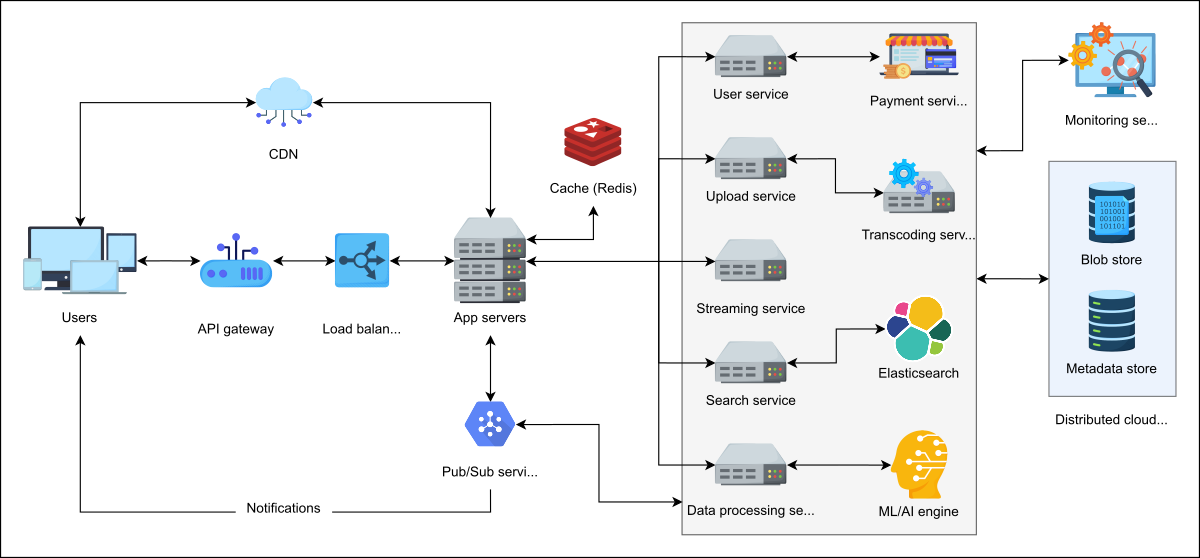
\includegraphics[width=0.5\textwidth]{Images/chapter_45/section_4733042868224000/4815189596045312.png}
 \caption{An overview of Spotify’s scalable System Design}
\end{figure}

\subsubsection{Key system components and services}\label{aOvWn9SJb8b05FHe-xSTf}
\\
Here's how Spotify processes user requests and ensures scalability:

\begin{itemize}
\item
\protect\phantomsection\label{Aweb40jJPumDk3DCB5yD4}
\textbf{API Gateway:} Acts as the entry point, authenticating user requests.
\item
\protect\phantomsection\label{E4UexU9WKI7EykHNBA74p}
\textbf{Load Balancer:} Distributes requests evenly across application servers to handle large volumes of traffic.
\item
\protect\phantomsection\label{Yyh1YnCdheDy5LJ_Ai5kC}
\textbf{Messaging Queue:} User interactions (e.g., playing songs, creating playlists) are sent to a queue (like Pub/Sub or Kafka). This queue distributes data to various microservices for tasks such as generating recommendations or creating wrapped summaries. This allows the data to be processed asynchronously, improving scalability and availability.
\end{itemize}
\\
This asynchronous approach enhances scalability and availability, ensuring Spotify's system can handle traffic spikes and real-time demands.
\\
Spotify's microservices architecture supports various tasks:

\begin{itemize}
\item
\protect\phantomsection\label{p-riayDpknpFBldSUGZT3}
\textbf{User service:} Manages user data, including preferences and subscriptions, with connections to a payment service for subscription verification.
\item
\protect\phantomsection\label{dmlQnLYLbfyS9qMIDJUNs}
\textbf{Upload service:} Ingests new content from artists.~
\item
\protect\phantomsection\label{tCU6gPFV85LRABD4nSrNO}
\textbf{Transcoding service:} Converts uploaded files into streaming-compatible formats, storing them in cloud-based blob storage (and metadata into an SQL database).
\item
\protect\phantomsection\label{3EvDfJzCLdgogpMYFkjVQ}
\textbf{Streaming service:} Delivers content to users via a content delivery network (CDN), minimizing latency.
\item
\protect\phantomsection\label{qNqaet32VKeUwxNMvxoUl}
\textbf{Search service:} Enables fast lookups using Elasticsearch.
\item
\protect\phantomsection\label{_YmJQXt3dKZZAC8uA5wcv}
\textbf{Processing service:} Powers recommendations and wrapped summaries using advanced machine learning models.
\item
\protect\phantomsection\label{d05qTmv4Yfj5rlPA3KVw9}
\textbf{Monitoring service:} Monitors the overall system's health and alerts in case of errors, failures, etc.
\end{itemize}

\subsubsection{Distributed databases}\label{589uHY8tV51R2sPuWNYNu}
\\
Spotify employs multiple database types:

\begin{itemize}
\item
\protect\phantomsection\label{r-He-pHPDRR-CCUeTj2fr}
\textbf{Blob storage:} Stores tracks, podcasts, and audiobooks.
\item
\protect\phantomsection\label{_yZyDdXC5qXqLjvVRX9Q_}
\textbf{SQL databases:} Store user metadata, such as account details.
\item
\protect\phantomsection\label{C3b5QlpqoSzWUUWLwbRbd}
\textbf{NoSQL databases:} Handle activity data, including listening history, playlists, and preferences.
\end{itemize}

\subsubsection{System Design for Spotify Wrapped}\label{zerAuJJCHV5AdzE0PaHWT}
\\
Let's explore how data processing services handle such a massive amount of data at scale to create personalized Spotify Wrapped experiences.
\\
Spotify uses the ETL (Extract, Transform, Load) process: \textbf{Extract} defines how data is collected, \textbf{Transform} covers how data is processed and turned into features, and \textbf{Load} specifies where data is stored for efficient retrieval. They also use reverse ETL to create Wrapped from the processed data.
\\
\paragraph{Data collection or ingestion (Extract)}\label{HdsWf6Trk2zeJM49OTnwD}
\\
A \textbf{data collection service} collects data from data resources (databases) and passes it to tools like Kafka or Pub/Sub to stream and make it available for immediate processing.
\\
\paragraph{Data processing (Transform)}\label{tdCYFGtrU3jm2IcPwnDtr}
\\
The data from the ingestion layer is fed to the processing layer, where the batch processor runs on massive data, aggregating users' year-long listening tasks and generating insights. Spotify utilizes Google Cloud Bigtable to efficiently manage its extensive time-series data and user listening history, optimizing it for rapid data aggregation over specific time frames.~
\\
In 2019, Spotify's use of Bigtable and BigQuery for data processing resulted in processing 5 times the data while reducing the overall cost by 25 percent.
\\
Spotify can quickly compile user-level insights by structuring data storage to minimize shuffling (reducing the need to move data between nodes, which can be time-consuming and resource-intensive) during processing.
\begin{quote}
\textbf{Note:} The following illustration is an in-depth exploration of how data processing services process data and transform it into a personalized Wrapped.
\end{quote}

\begin{figure}[htbp]
 \centering
 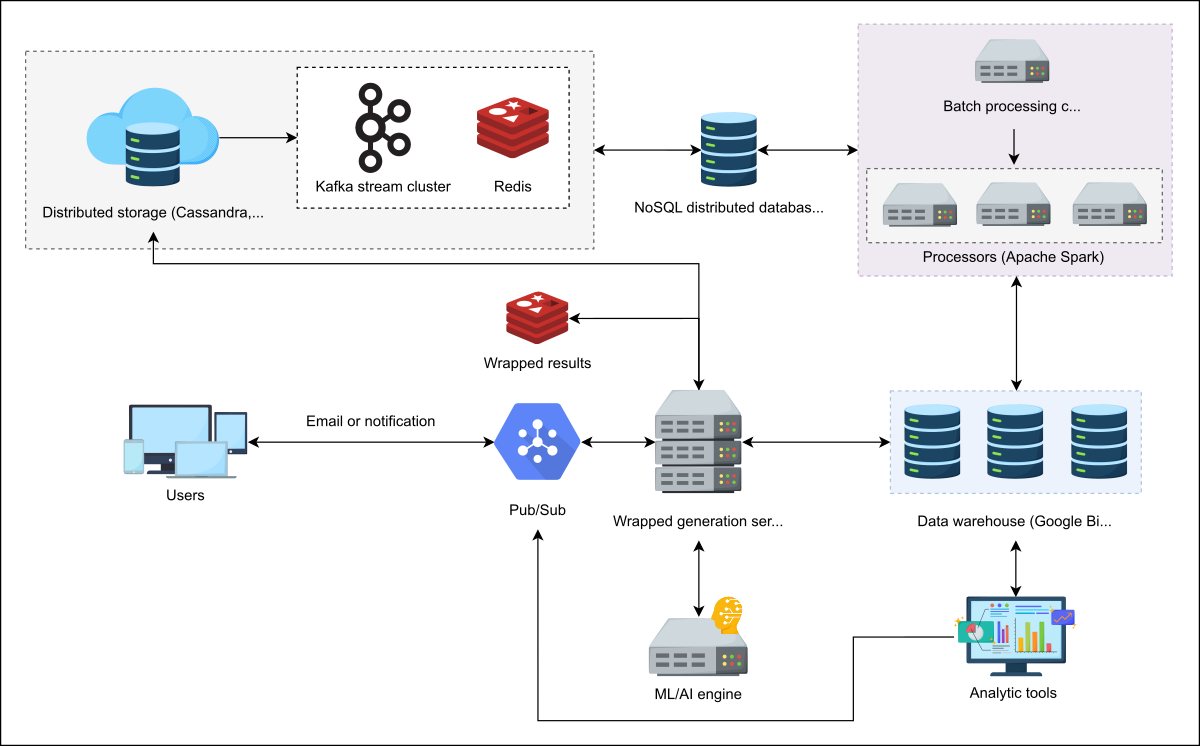
\includegraphics[width=0.5\textwidth]{Images/chapter_45/section_4733042868224000/5847017320742912.png}
 \caption{A detailed design of data processing for Spotify Wrapped}
\end{figure}

\paragraph{Data warehousing (Load)}\label{CDFbYJbdENTpHrkxp7iCb}
\\
Apache Spark and other big data frameworks process this data at scale, and the results are stored in data warehouses, such as Google BigQuery.
\\
\paragraph{Wrapped creation and personalization (Reverse ETL)}\label{l7CmYhP-5VojUPmwz-dwG}
\\
Finally, data visualization tools and services aggregate this processed data, allowing Wrapped summaries to be sent to the user in real time through APIs. Cloud services ensure low latency, high availability, and scalability across Spotify's global infrastructure.
\\
The Wrapped summaries are sent to users via Email or in-app notifications through the Pub/Sub service.
\begin{quote}
\textbf{Note:} Spotify Wrapped is all about personalization, done by utilizing advanced machine learning algorithms. The ML engine uses collaborative filtering(A filtering technique to recommend content based on the behavior of similar users or items.), content-based filtering(A filtering technique to recommend content based on similarities between items or content based on metadata and content features.), and a hybrid model, mostly the best of both, to generate personalized Wrapped for each user.
\end{quote}
\\
For 2019 Wrapped, Spotify processed decade-long user data utilizing Bigtable. A similar data processing pattern for a year-long dataset is shown below:

\begin{figure}[htbp]
 \centering
 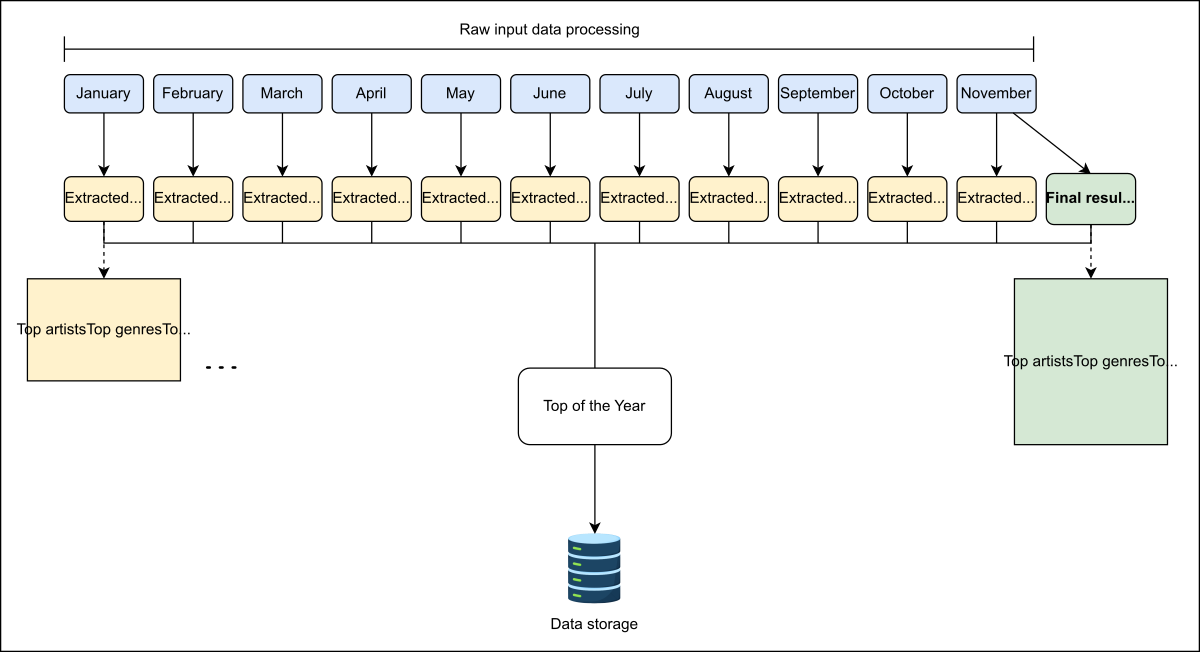
\includegraphics[width=0.5\textwidth]{Images/chapter_45/section_4733042868224000/5695587628744704.png}
 \caption{The architecture of data pipelines [source: Spotify]}
\end{figure}

\subsubsection{Front-end animations in Spotify Wrapped}\label{DJmtvPIDKfYL197MagyIj}
\\
The front-end experience for Spotify Wrapped plays a crucial role in driving user engagement. The design of the Wrapped interface transforms raw data into fun, shareable content.
\\
Spotify Wrapped's front-end elements include:
\\
\paragraph{Visual and interactive features}\label{kdGXxm7pzKR55q-TI6tDZ}

\begin{itemize}
\item
\protect\phantomsection\label{jqmrLed0pvBJT4c21ulro}
\textbf{Personalized visualizations:} Insights are displayed as animated reels or cards.
\item
\protect\phantomsection\label{Cn4lgIFD3AH7J231dCya6}
\textbf{NLP-powered content:} Uses natural language processing to generate captions and labels for animations.
\end{itemize}
\\
\paragraph{Feature highlights}\label{OHV9VsN-pZOVoZR2HbfWl}

\begin{itemize}
\item
\protect\phantomsection\label{BhwQ2pdaslmezZvaVKAi_}
\textbf{Audio Aura (2021):} Colors representing listening intensity for different genres.
\item
\protect\phantomsection\label{8HTW9xPTjlb6oHKuhWK2A}
\textbf{Sound Town (2023):} Mapped users' tastes to fictional cities, creating playful, shareable visuals.
\end{itemize}
\\
These interactive features enhance user engagement, turning data into delightful experiences.

\begin{figure}[htbp]
 \centering
 
\includegraphics[width=0.15\textwidth]{Images/chapter_45/section_4733042868224000/4820040207958016.png}
 \caption{2023 Sound Town [Source: Spotify]}
\end{figure}

\subsection{What we can learn from Spotify~}\label{iKFYKqWCMAHD4Ruf0k5Go}
\\
Here are 4 key takeaways from Spotify's approach to delivering a seamless Wrapped experience each year:

\begin{enumerate}
\item
\protect\phantomsection\label{HmTp-ZAZhG4ULoJiMy5Gn}
A robust, scalable System Design is the backbone of Wrapped. It handles huge data volumes by separating real-time and batch-processing content, ensuring fast data access and reliable yearly insights.
\item
\protect\phantomsection\label{ejyygQYdu972MV-anogIq}
Using solutions like Bigtable and BigQuery, Spotify minimizes data shuffling and enables efficient aggregation, providing users with quick, user-level insights for millions.
\item
\protect\phantomsection\label{_Bmbf5Ua4mrbqLkANJB49}
Advanced machine learning models help Spotify deliver Wrapped's unique, personalized insights by analyzing patterns in listening data.
\item
\protect\phantomsection\label{yW01UvTkJIivPc6WPWKkt}
By employing auto-scaling and load balancing, Spotify can smoothly manage the surge in Wrapped engagement.
\end{enumerate}

\subsection{What's next for Spotify Wrapped?}\label{xQmIFQTpkANu2zXd0qY1m}
\\
As Spotify Wrapped continues to scale year after year, it offers a glimpse into the complex System Design that powers real-world applications at a massive scale.~
\\
Spotify's developers continually add new features and insights to enhance the user experience, making it challenging to predict what's coming next. However, we can expect AI to level up the Wrapped experience through features like:

\begin{itemize}
\item
\protect\phantomsection\label{hvFrXScJ3RLZO-yCpiaUp}
Interactive, real-time playlists that evolve based on a user's Wrapped experience.~
\item
\protect\phantomsection\label{zbGVpkHNr9P31Aus8y5wu}
AI-driven music DNA visualizations breaking down listening habits into dynamic, shareable formats.
\item
\protect\phantomsection\label{KbzelczrjhSfAgrsezXpf}
Leveraging GenAI to create unique soundtracks for users, blending favorite genres, moods, and artists into a custom composition.
\end{itemize}
\\
Spotify Wrapped highlights the importance of approaches like cloud-based data pipelines, advanced machine learning models, and auto-scaling for cost savings in System Design.
\\
\textbf{Disclaimer:} All technical information and design insights provided in this lesson are curated by our System Design experts to the best of their knowledge and based on available resources, including insights from Spotify's engineering blogs. While we strive for accuracy, some details may vary from Spotify's actual implementations and are intended for educational purposes only.

% End of section content